% ****************************************************************************************************
% Chapter 2: The Competition and the Discovery
% ****************************************************************************************************

\chapter{The Competition and the Discovery}
\label{ch:discovery}

In late 2025, the Laitinen-Fredriksson Foundation launched a Kaggle competition called Triagegeist. The task was straightforward: given a set of patient features, predict the ESI acuity level assigned at triage. The prize was research funding; the evaluation was based on a scoring rubric spanning clinical relevance, technical quality, documentation, insight, and novelty. A Kaggle notebook had to run end-to-end, and a written submission had to accompany it.

This chapter describes what happened when I started looking at the data.

\section{The Dataset}

The competition organisers provided four CSV files \citep{triagegeist2025}. The \texttt{train.csv} file contained 80,000 labelled rows, each describing a single ED visit with vital signs, demographics, and a target column \texttt{triage\_acuity} taking integer values from 1 to 5. The \texttt{test.csv} file contained 20,000 unlabelled rows with the same features. Two auxiliary files provided joinable information: \texttt{chief\_complaints.csv} contained a free-text \texttt{chief\_complaint\_raw} column and a categorical \texttt{chief\_complaint\_system} label (one of fourteen body-system categories), while \texttt{patient\_history.csv} contained twenty-five binary comorbidity flags named \texttt{hx\_*} and a summary \texttt{num\_comorbidities} count.

The class distribution in the training set is shown in Figure~\ref{fig:class-distribution-kaggle}. ESI-3 dominates at 36.1\%, ESI-4 follows at 28.8\%, and the extremes are relatively small: 4.0\% for ESI-1 and 14.2\% for ESI-5. This is reasonable enough at first glance. Real EDs do see more moderate-acuity patients than critical ones, and the shape of the distribution did not, initially, raise any alarms.

\begin{figure}[htbp]
 \centering
 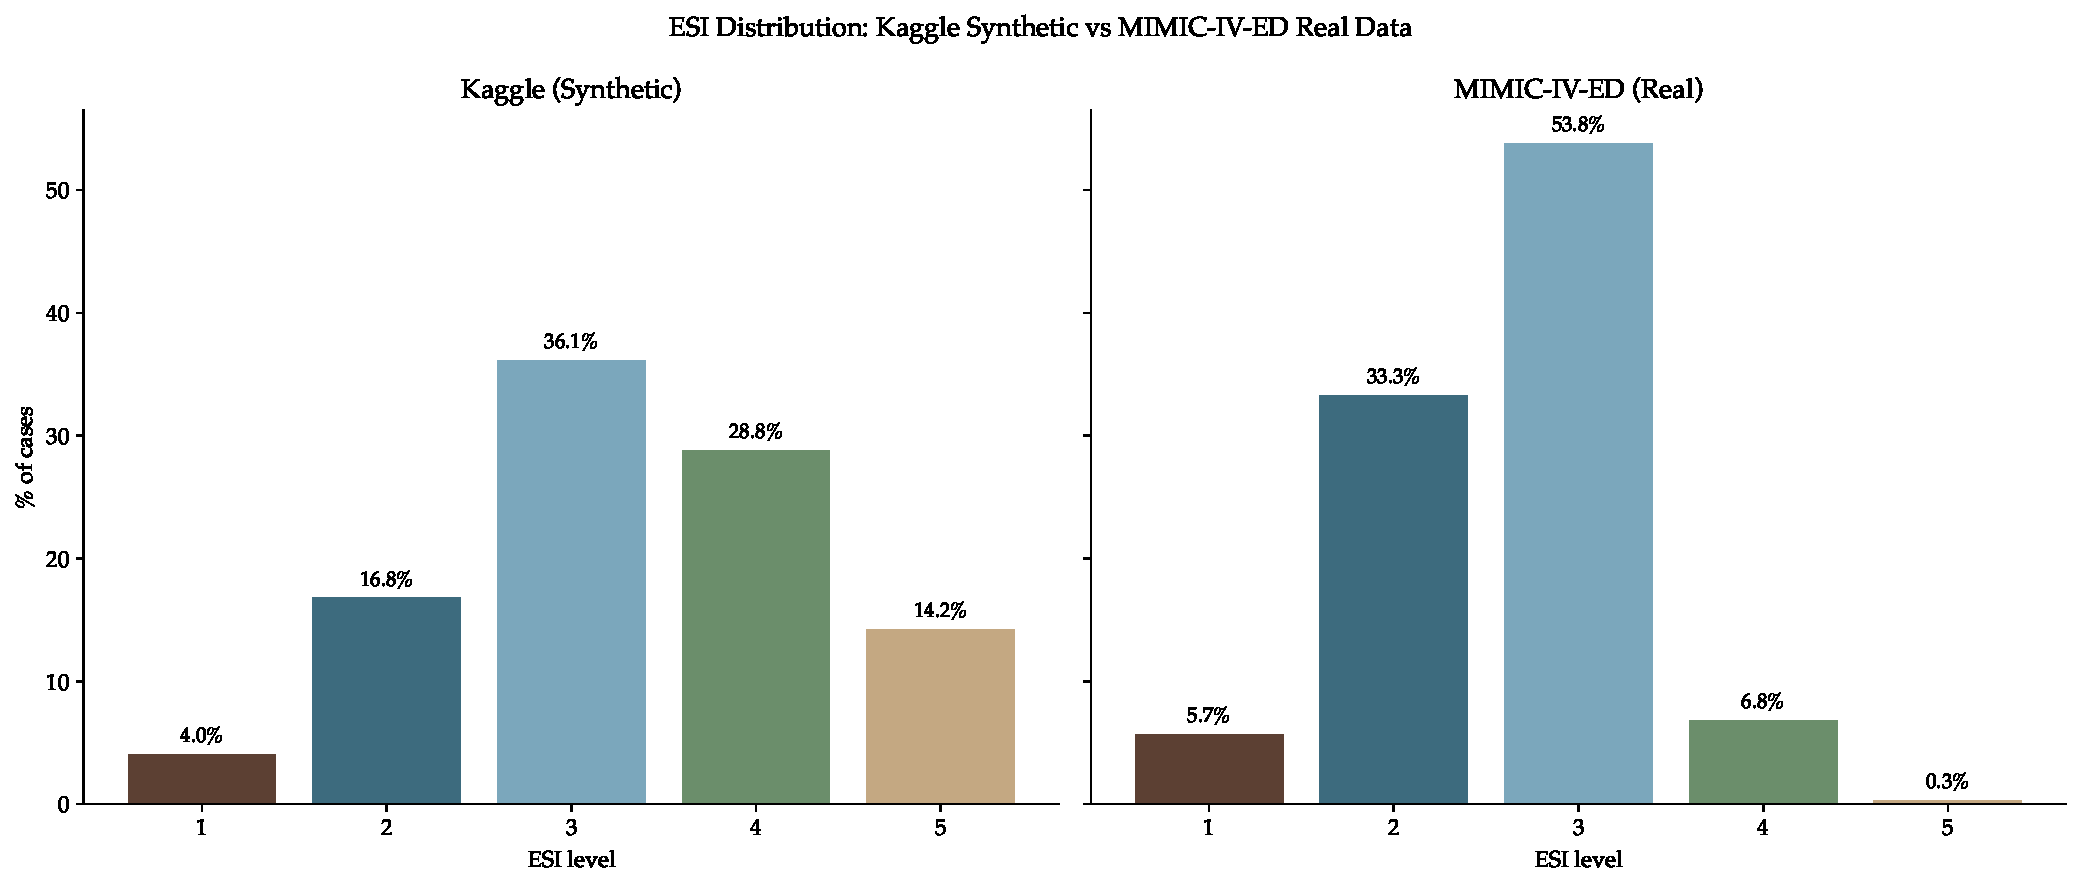
\includegraphics[width=\textwidth]{figures/class_distribution_comparison.pdf}
 \caption[Class distribution: Kaggle synthetic vs MIMIC-IV-ED]{Class distribution of ESI acuity levels in the Kaggle competition data (left) and in MIMIC-IV-ED (right). The synthetic distribution is roughly bell-shaped around ESI-3. The real-world distribution is strikingly different: ESI-3 is even more dominant at 53.8\%, but the extremes collapse. ESI-1 is rare at 5.7\%, ESI-4 at 6.8\%, and ESI-5 nearly absent at 0.3\%. The differences between these two distributions were the first clue that the competition dataset was synthetic.}
 \label{fig:class-distribution-kaggle}
\end{figure}

\section{The First Model}

My first attempt followed the standard Kaggle recipe. I joined all four tables on \texttt{patient\_id}, engineered some basic features (shock index, mean arterial pressure, pulse pressure, missingness flags), and trained a LightGBM classifier with five-fold stratified cross-validation. The macro F1 score was 0.873. This is a perfectly respectable number for a five-class problem with this level of imbalance, and I initially assumed this would be roughly the ceiling of honest tabular modelling.

\begin{notebox}[What is Macro F1?]
Macro F1 is the arithmetic mean of per-class F1 scores, where F1 is the harmonic mean of precision and recall. ``Macro'' means I average the per-class scores equally, so a rare class contributes as much as a common one. This is the right choice for imbalanced ordinal problems like mine: I care about the rare ESI-1 patients as much as the common ESI-3 ones, and possibly more.
\end{notebox}

The next step was to add the text. Many Kaggle participants publishing public notebooks were evidently using the \texttt{chief\_complaint\_raw} column, and the competition rubric rewarded using all available data. I encoded the chief complaint text using sentence-transformers' \texttt{all-MiniLM-L6-v2} model \citep{reimers2019sentence}, producing 384-dimensional embeddings for each complaint, and concatenated these to the tabular features.

The result was strange. Macro F1 jumped to 0.998. Essentially perfect.

A jump from 0.87 to 0.998 from adding text is not how machine learning works. Not on a real clinical problem, at least. Text embeddings on chief complaints should add useful signal, the word ``chest pain'' carries different information than ``ankle sprain'', but they should not make the task trivial. I looked more carefully.

\section{Looking at the Text}

I pulled out a hundred random rows for each ESI level and started reading the complaints. The pattern was immediate.

ESI-1 and ESI-2 complaints contained words like \emph{severe}, \emph{acute}, \emph{massive}. ESI-3 complaints used \emph{moderate} as a modifier. ESI-4 and ESI-5 complaints used \emph{mild}, \emph{minor}, and \emph{stable}.

This was suspicious. Real chief complaints, as written by triage nurses, do not follow such a neat lexical partition. A triage note for a critically ill patient might read ``63M c/o chest pain radiating to L arm'' with no adjective at all. A mild case might read ``48F, sore throat x 3 days, no fever, requests test.'' The severity-adjective vocabulary is standard English, but its correlation with triage level in real data is weak and inconsistent.

I decided to quantify the pattern. For each severity-related keyword, I computed the percentage of rows at each ESI level whose chief complaint text contained that keyword. The result is shown in Figure~\ref{fig:keyword-leakage}.

\begin{figure}[htbp]
 \centering
 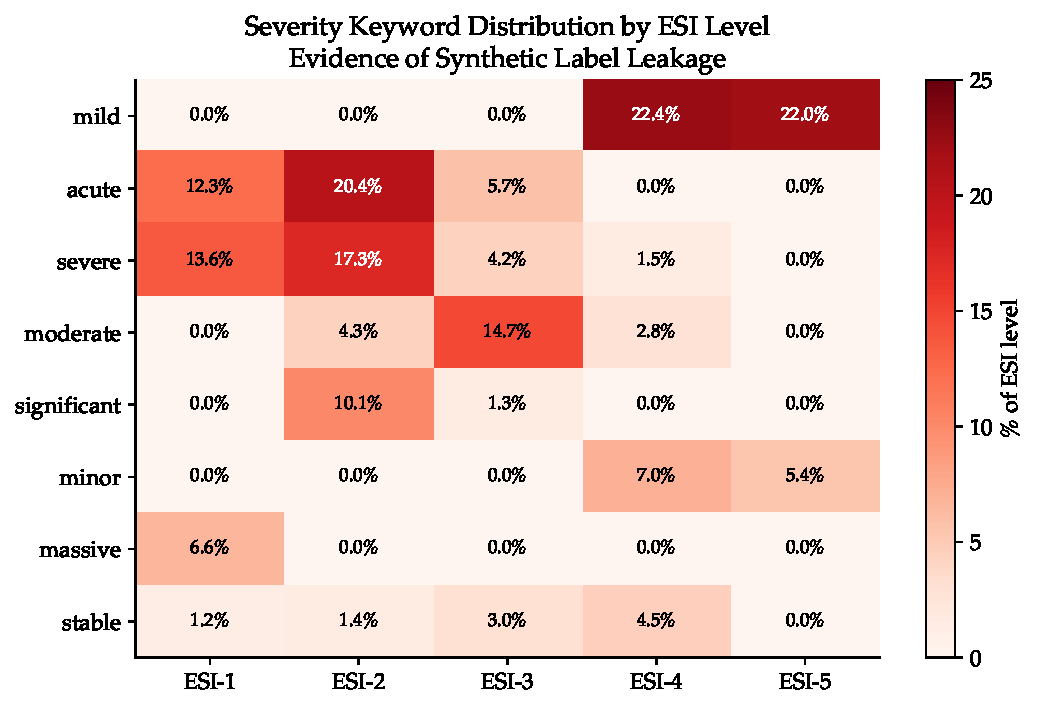
\includegraphics[width=0.85\textwidth]{figures/keyword_leakage_heatmap.pdf}
 \caption[Severity keyword distribution by ESI level]{Percentage of chief complaint texts at each ESI level containing each severity-related keyword. The distributions are near-disjoint: ``mild'' never appears in ESI-1, 2, or 3 but appears in 22\% of ESI-4 and ESI-5 cases. ``Massive'' appears only in ESI-1. ``Moderate'' is concentrated in ESI-3. ``Severe'' is concentrated in ESI-1 and ESI-2. This pattern is not plausible in real clinical text and is strong evidence that the dataset is synthetically generated with labels encoded in the text.}
 \label{fig:keyword-leakage}
\end{figure}

The pattern was unmistakable. The keyword distributions were effectively non-overlapping across ESI levels. In real ED notes, a word like ``severe'' might appear across all acuity levels, a patient with severe but chronic pain may not be acutely ill, while a patient in critical condition might have no adjectives in their note at all. But in this dataset, the words partitioned the levels almost cleanly.

This is what label leakage looks like. The features contained information about the label that would not be available in a real deployment. In this case, the leakage was not subtle: the labels had been encoded directly into the text during data generation.

\begin{notebox}[What Is Label Leakage?]
Label leakage occurs when features available at prediction time contain information about the target that would not realistically be available in deployment. The canonical example is predicting hospital readmission using features collected \emph{after} the readmission occurred. In my case, a real triage nurse writing a chief complaint does not systematically encode the acuity level in their word choice, the two are correlated in the training data because the dataset was synthetically generated with that encoding built in.

Models trained on leaky features appear to perform well in development and fail in deployment. The high accuracy is an artefact of the data, not evidence of useful learning.
\end{notebox}

\section{The Smoking Gun: Exact Matches}

The keyword analysis was strong evidence but not proof. A reviewer might argue, reasonably, that complaint text correlated with acuity in the real world more than I was crediting. I wanted a test that could not be explained away.

I looked at unique chief complaint strings. There were 4,949 unique complaints in the training set and 4,412 in the test set. If the data were real, each patient's complaint would be an individual utterance written by a specific nurse in a specific moment. There would be recurring phrases, ``chest pain'' appears often, but the exact string, character for character, would rarely repeat.

In this dataset, 4,382 of the 4,412 unique test complaints appeared \emph{verbatim} in the training set. That is 99.3\% of unique complaints, and 99.8\% of test rows.

I computed the majority label for each repeated complaint in the training set, then applied it to the test rows with matching complaints. The accuracy was 99.93\%.

A lookup table, with no machine learning whatsoever, would score above 0.999 on this competition. The synthetic data generator had produced a finite vocabulary of complaint strings, and each string had a deterministic relationship with its acuity label.

\begin{figure}[htbp]
 \centering
 \begin{lstlisting}[language=Python, caption={The exact-match analysis. Three lines of pandas produced the smoking gun.}]
train_complaints = set(df_train['chief_complaint_raw'].unique())
test_complaints = set(df_test['chief_complaint_raw'].unique())
overlap = train_complaints & test_complaints
print(f"{len(overlap)/len(test_complaints)*100:.1f}% of test complaints "
 f"appear verbatim in training")
# Output: 99.3% of test complaints appear verbatim in training
 \end{lstlisting}
 \label{fig:exact-match-code}
\end{figure}

\section{The Categorical System Column Has No Signal}

If the text column encoded the label directly, perhaps the categorical \texttt{chief\_complaint\_system} column (one of fourteen body-system categories like ``cardiovascular'' or ``respiratory'') carried the real clinical signal. I tested this with a chi-squared test of independence on the cross-tabulation of \texttt{chief\_complaint\_system} and \texttt{triage\_acuity}.

The chi-squared statistic was 59.8 with 52 degrees of freedom, giving $p = 0.213$. Under conventional significance thresholds, this is consistent with the two variables being statistically independent. Knowing which body system a patient's complaint fell under, cardiovascular, respiratory, neurological, genitourinary, and so on, gave essentially no information about their triage acuity.

This was another clue about how the synthetic data had been generated. A real ED dataset would show strong associations: cardiovascular complaints skew toward higher acuity because of the prevalence of cardiac emergencies; minor orthopaedic complaints skew toward lower acuity. The absence of this association suggests that the body-system label was sampled independently from the acuity in the data generation process, while the severity-modifier vocabulary was conditioned on it.

\section{What the Leaderboard Actually Measures}

I now had a clear picture of the competition. The dataset was synthetically generated. The \texttt{chief\_complaint\_raw} column had labels encoded into its severity-modifier vocabulary. The categorical \texttt{chief\_complaint\_system} column was independent of the label. Any competitor who used the raw text would achieve macro F1 above 0.99. Any competitor who used only the tabular features and comorbidity history would plateau around 0.87.

The Kaggle leaderboard, in other words, was not measuring clinical prediction quality. It was measuring whether competitors had noticed the synthetic text encoding. This is not a useful distinction between methods. Any reasonably competent NLP pipeline would recover it; any rigorous clinical ML system would ignore the leakage and score lower. The leaderboard would reward pattern recovery, not science.

I was now faced with a decision.

\section{The Pivot}

The competition was rubric-graded, not leaderboard-graded. The formal scoring assigned points across five dimensions: clinical relevance (25), technical quality (30), documentation (20), insight and findings (15), and novelty (10). Leaderboard position was not in the rubric. This changed the strategic calculation considerably.

I could play the leaderboard game: use the text exploit, score 0.999, and be one of dozens of competitors with an indistinguishable result. Or I could treat the competition as an invitation to do real clinical machine learning, validate the methodology on a real dataset, and use the synthetic leakage as a case study in its own right. The second path required substantially more work and carried no guarantee of winning, but it was the only one that would produce science.

I chose the second path. The specific choice involved three decisions.

First, I would develop and validate all methodology on a real clinical dataset with real ED patients. This meant MIMIC-IV-ED, the publicly available Beth Israel Deaconess Medical Center dataset, which required credentialed access through PhysioNet but contained 418,100 real ED visits with detailed triage information. Chapter~\ref{ch:mimic} describes this pivot in detail.

Second, I would still submit a competitive Kaggle notebook. But the notebook would be a narrative document, not a leaderboard optimiser. It would present the leakage discovery as a first-class finding, show both the text-exploit and the honest tabular baselines, and use the real clinical validation as the main evidence for methodological quality. The Kaggle competition would be won, if at all, on the rubric.

Third, I would treat the synthetic leakage finding as a contribution in its own right. The specific mechanism, adjective vocabulary encoded by acuity level, near-total verbatim overlap between train and test, independent body-system labelling, was not obvious until I looked carefully. Documenting the investigation might be useful to future researchers working with similar synthetic clinical datasets.

\begin{highlightbox}
The remainder of this report is almost entirely about what happened after the pivot. The Kaggle submission itself is described briefly in Chapter~\ref{ch:explainability}; all the scientific content from Chapter~\ref{ch:mimic} onward concerns the real clinical data. The synthetic competition and its leakage discovery serve as the motivation and framing for that work, not as its subject.
\end{highlightbox}

\section{A Note on What I Did Not Do}

I considered, but did not pursue, two alternative strategies that deserve acknowledgement.

The first was to write up the leakage as a Kaggle Discussion post and alert other participants. I chose not to do this because the competition was still in its active submission window, and posting the finding publicly would have given a competitive advantage to participants who had not yet discovered the issue. I planned to share the full analysis after the submission deadline, both on the Kaggle forum and in this report, which I judged to be the correct balance between competitive fairness and scientific openness.

The second was to submit only the text-exploit model and treat the competition as a pure leaderboard exercise. I rejected this because it would have produced no useful work product, no portfolio artefact, no scientific contribution, nothing to show at the end except a leaderboard rank on a flawed benchmark. The rubric-graded structure of the competition made it much more valuable to do the real work.

With that said, let me turn to the real work: obtaining and analysing clinical data from Beth Israel Deaconess Medical Center.
